\documentclass[]{book}
\usepackage{lmodern}
\usepackage{amssymb,amsmath}
\usepackage{ifxetex,ifluatex}
\usepackage{fixltx2e} % provides \textsubscript
\ifnum 0\ifxetex 1\fi\ifluatex 1\fi=0 % if pdftex
  \usepackage[T1]{fontenc}
  \usepackage[utf8]{inputenc}
\else % if luatex or xelatex
  \ifxetex
    \usepackage{mathspec}
  \else
    \usepackage{fontspec}
  \fi
  \defaultfontfeatures{Ligatures=TeX,Scale=MatchLowercase}
\fi
% use upquote if available, for straight quotes in verbatim environments
\IfFileExists{upquote.sty}{\usepackage{upquote}}{}
% use microtype if available
\IfFileExists{microtype.sty}{%
\usepackage{microtype}
\UseMicrotypeSet[protrusion]{basicmath} % disable protrusion for tt fonts
}{}
\usepackage{hyperref}
\hypersetup{unicode=true,
            pdftitle={Mind, Brain, Body},
            pdfauthor={Emily Towner},
            pdfborder={0 0 0},
            breaklinks=true}
\urlstyle{same}  % don't use monospace font for urls
\usepackage{natbib}
\bibliographystyle{apalike}
\usepackage{longtable,booktabs}
\usepackage{graphicx,grffile}
\makeatletter
\def\maxwidth{\ifdim\Gin@nat@width>\linewidth\linewidth\else\Gin@nat@width\fi}
\def\maxheight{\ifdim\Gin@nat@height>\textheight\textheight\else\Gin@nat@height\fi}
\makeatother
% Scale images if necessary, so that they will not overflow the page
% margins by default, and it is still possible to overwrite the defaults
% using explicit options in \includegraphics[width, height, ...]{}
\setkeys{Gin}{width=\maxwidth,height=\maxheight,keepaspectratio}
\IfFileExists{parskip.sty}{%
\usepackage{parskip}
}{% else
\setlength{\parindent}{0pt}
\setlength{\parskip}{6pt plus 2pt minus 1pt}
}
\setlength{\emergencystretch}{3em}  % prevent overfull lines
\providecommand{\tightlist}{%
  \setlength{\itemsep}{0pt}\setlength{\parskip}{0pt}}
\setcounter{secnumdepth}{5}
% Redefines (sub)paragraphs to behave more like sections
\ifx\paragraph\undefined\else
\let\oldparagraph\paragraph
\renewcommand{\paragraph}[1]{\oldparagraph{#1}\mbox{}}
\fi
\ifx\subparagraph\undefined\else
\let\oldsubparagraph\subparagraph
\renewcommand{\subparagraph}[1]{\oldsubparagraph{#1}\mbox{}}
\fi

%%% Use protect on footnotes to avoid problems with footnotes in titles
\let\rmarkdownfootnote\footnote%
\def\footnote{\protect\rmarkdownfootnote}

%%% Change title format to be more compact
\usepackage{titling}

% Create subtitle command for use in maketitle
\providecommand{\subtitle}[1]{
  \posttitle{
    \begin{center}\large#1\end{center}
    }
}

\setlength{\droptitle}{-2em}

  \title{Mind, Brain, Body}
    \pretitle{\vspace{\droptitle}\centering\huge}
  \posttitle{\par}
    \author{Emily Towner}
    \preauthor{\centering\large\emph}
  \postauthor{\par}
      \predate{\centering\large\emph}
  \postdate{\par}
    \date{2020-03-27}

\usepackage{booktabs}
\usepackage{amsthm}
\makeatletter
\def\thm@space@setup{%
  \thm@preskip=8pt plus 2pt minus 4pt
  \thm@postskip=\thm@preskip
}
\makeatother

\begin{document}
\maketitle

{
\setcounter{tocdepth}{1}
\tableofcontents
}
\hypertarget{introduction}{%
\chapter{Introduction}\label{introduction}}

The Mind, Brain, Body study looks at how early caregiving experiences influence the emotional, cognitive, and brain development, as well as physical health and wellness.

The study also explores how the bacteria that live inside us (the microbiome) are connected to the development of our brains and bodies.

\hypertarget{consent}{%
\chapter{Consent}\label{consent}}

Once the parent and child come into the lab, seat them in the rainbow room on the couch for consenting.

Make some small talk - Ask the participant how they got here. If they have participated before in research. Offer them a bottle of water. Thank them for coming and for giving up their weekend to help science.

Tell the parent and child that the first thing you are going to do is go over all of the things they will do today, and have them sign the consent forms.

Speak to them and direct them through the whole process.

Things you will do in the lab

\begin{itemize}
\tightlist
\item
  Stick stickers on you to measure heart rate, sweat, stomach muscles.
\item
  Sit with parent and talk about fun things and hard things (filming).
\item
  Parent stays in room and answers more questions.
\item
  Child goes next door to play computer games (look at pictures, watch movies). Some of the movies and pictures will be a little bit scary, others sad, others boring.
\item
  One of the games involves a loud annoying noise, we will adjust it for you.
\item
  You will also do some other games on paper and pencil - like puzzle and word games
\item
  You will answer some questionnaires
\item
  We will also measure your height, weight, and waist circumference.
\item
  We will take three biological samples:

  \begin{itemize}
  \tightlist
  \item
    Hair - stress hormones
  \item
    Saliva - microbiome
  \item
    Blood - immune - wear goggles
  \end{itemize}
\item
  Do you get sick or dizzy when you see blood or hurt yourself?
\item
  If we need to, can we prick two fingers?
\item
  When you are done with all of that, you will get a big prize, then we will pay you and you will go home.
\item
  You will get \$45 for the work you put in today.
\end{itemize}

Things you will do at home

Child

\begin{itemize}
\tightlist
\item
  Poop sample - microbiome
\item
  Stool scale
\item
  Memory game - to see what you remember from lab.
\end{itemize}

Parent

\begin{itemize}
\tightlist
\item
  24 hour food recall
\end{itemize}

When you complete the poop sample and the games at home, we will pay you another \$20 in the form of a giftcard.

Things to know

You are a volunteer, which means that you do not have to do anything, or say anything that makes you uncomfortable. We would like you to try everything you can, and to do your best, but if there are things you absolutely do not want to do, just tell us, that is o.k.

We keep your participation confidential - ID number.

We want you to come in again in the future, so we will ask for some information so we can contact you in the future.

\emph{Sign consent/assent forms including DBS form and Contact Sheet}

\hypertarget{recruitment}{%
\chapter{Recruitment}\label{recruitment}}

Pre-Screening

\begin{enumerate}
\def\labelenumi{\arabic{enumi}.}
\tightlist
\item
  Check if participant is in Recruitment Database

  \begin{itemize}
  \tightlist
  \item
    If not, add them to the Recruitment Database
  \end{itemize}
\item
  Check if participant is in ID Drive

  \begin{itemize}
  \tightlist
  \item
    If yes, check if they have a Screener ID
  \item
    If not, assign them a Screener ID once contact has been established based on the next available Screener ID \# in REDCap and proceed with screening
  \item
    If yes, proceed with screening under existing Screener ID in REDCap
  \end{itemize}
\end{enumerate}

Screening

\begin{enumerate}
\def\labelenumi{\arabic{enumi}.}
\item
  To screen a new participant click ``Add / Edit Records''
\item
  Click to enter a new Subject ID

  \begin{itemize}
  \tightlist
  \item
    Make sure Arm 1: Recruitment is selected
  \end{itemize}
\item
  Type ``SMBB\#'' (Screener ID) to create a record and hit ``Enter''

  \begin{itemize}
  \tightlist
  \item
    Make sure to link the participants Screener ID and their name on the \textbf{ID Drive ONLY}
  \item
    Before creating a new record, be sure to check the ID Drive to see if the participant already has an existing Screener ID
  \item
    If a record exists, add a new instance of the screen instead of creating a new record
  \end{itemize}
\item
  The screening arm contains two parts

  \begin{itemize}
  \tightlist
  \item
    The screen
  \item
    The wave1\_status

    \begin{itemize}
    \tightlist
    \item
      The wave1\_status is to be updated after the first and each subsequent contact
    \end{itemize}
  \end{itemize}
\item
  Click on the radio button in the ``screen'' row to screen the participant
\item
  Click ``Now'' to enter today's date and time
\item
  Select the appropriate choice to start the phone call and follow the skip logic.
\item
  Follow the skip logic to the end.

  \begin{itemize}
  \tightlist
  \item
    For items without a text field, write the information down in the Recruitment database (This identifying information cannot be on REDCap)
  \end{itemize}
\item
  Once done, select ``Complete'' and ``Save \& Exit Form''

  \begin{itemize}
  \tightlist
  \item
    The screen can be entered multiple times - for instance if there are multiple phone calls or contacts
  \item
    It is important to keep a record of all instances of contact
  \end{itemize}
\item
  Click the screen\_status radio button
\item
  Select the appropriate option
\end{enumerate}

\begin{itemize}
\tightlist
\item
  Contact - Participant needs to be re-contacted (add Recruitment Database \& ID Drive)
\item
  Ineligible - Participant not eligible for study
\item
  To Enroll - Participant to enroll (need to create subject ID, enter subject info, schedule participant, add to Recruitment Database, add to ID Drive)
\item
  Enrolled - Participant has been enrolled (all above have been completed)
\item
  To Remove - Participant wants to be removed
\end{itemize}

\begin{enumerate}
\def\labelenumi{\arabic{enumi}.}
\setcounter{enumi}{11}
\tightlist
\item
  Be sure to update the screen status after each contact
\end{enumerate}

\begin{itemize}
\tightlist
\item
  After 3 contacts (with no response) - review (time of day, contact method, etc.)
\end{itemize}

\begin{enumerate}
\def\labelenumi{\arabic{enumi}.}
\setcounter{enumi}{12}
\tightlist
\item
  If enrolled, proceed to pre-session checklist in the participant log
\end{enumerate}

Other Screening Information

Accessing Lists

To find out where participants are in the recruitment process, there are several lists.

\begin{enumerate}
\def\labelenumi{\arabic{enumi}.}
\item
  Click on ``Record Status Dashboard''
\item
  Participants who have been enrolled will be listed in the Enrollment - Wave 1 list
\item
  Participants in the process of recruitment will be listed in one of the 4 Recruitment lists

  \begin{itemize}
  \tightlist
  \item
    *These lists are populated based on the individuals ``Screen Status'' so be sure to update after each contact!
  \end{itemize}
\end{enumerate}

List Types

\begin{itemize}
\tightlist
\item
  Contact - List of individuals who need to be contacted or re-contacted (also includes waitlist)
\item
  Ineligible - Participants are ineligible but interested
\item
  To Enroll - Participants who have been screened and are eligible to enroll
\item
  To Remove - Participants who were not interested in being contacted for this or future research
\end{itemize}

\hypertarget{addressing-concerns}{%
\section{Addressing Concerns}\label{addressing-concerns}}

If a parent has a concern about the study before the session, send the email template:

\begin{itemize}
\tightlist
\item
  {[}MBB - CONCERNS{]}
\end{itemize}

\hypertarget{final-checklist}{%
\chapter{Final Checklist}\label{final-checklist}}

\hypertarget{generating-report-cards}{%
\section{Generating Report Cards}\label{generating-report-cards}}

\begin{enumerate}
\def\labelenumi{\arabic{enumi}.}
\tightlist
\item
  Open a participant data folder
\end{enumerate}

\begin{figure}
\centering
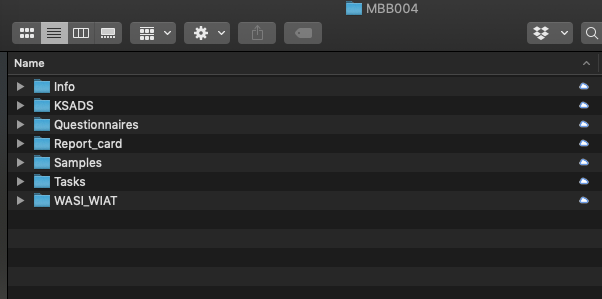
\includegraphics{images/final_checklist/report_cards/1.png}
\caption{}
\end{figure}

\begin{enumerate}
\def\labelenumi{\arabic{enumi}.}
\setcounter{enumi}{1}
\tightlist
\item
  Navigate to the report card folder and rename the template file - MBB999 to the relevant participant - and open the file
\end{enumerate}

\begin{figure}
\centering
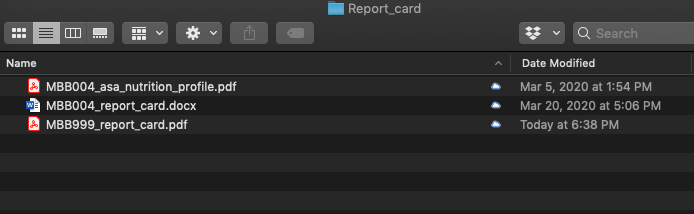
\includegraphics{images/final_checklist/report_cards/2.png}
\caption{}
\end{figure}

\begin{enumerate}
\def\labelenumi{\arabic{enumi}.}
\setcounter{enumi}{2}
\tightlist
\item
  If an ASA nutrition report has been generated for this participant, delete page 4 of the pdf. If no ASA nutrition report has been generated, delete page 3 of the pdf.
\end{enumerate}

\begin{figure}
\centering
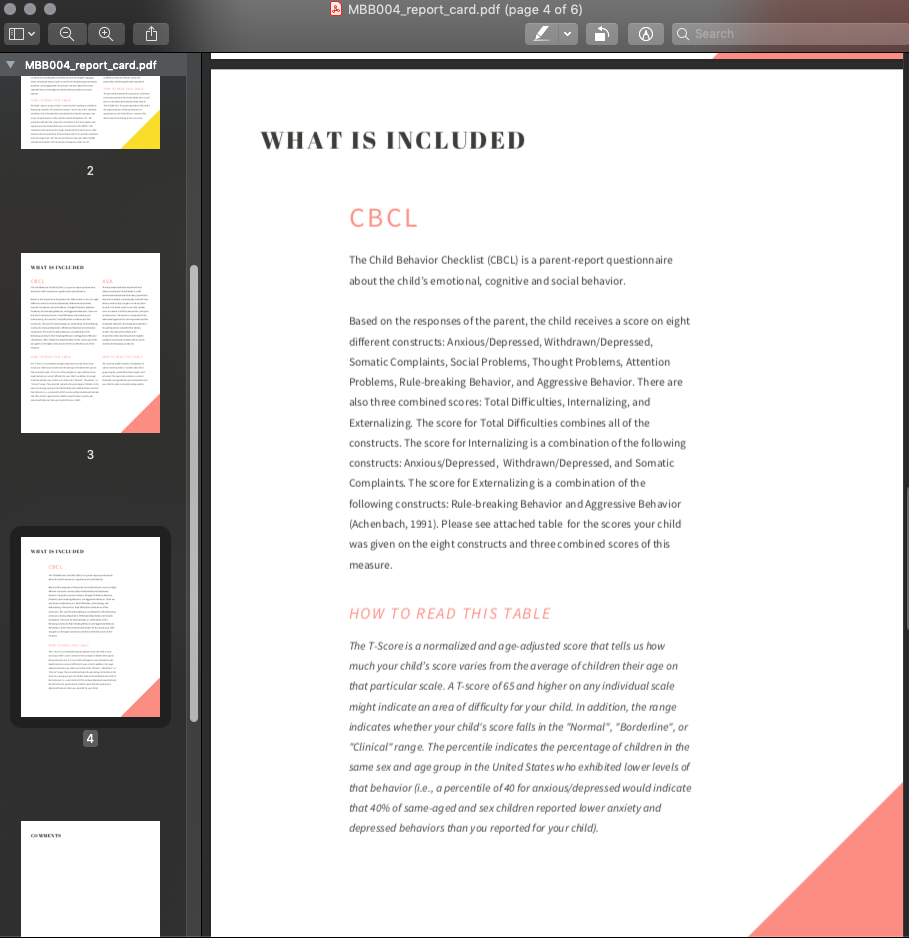
\includegraphics{images/final_checklist/report_cards/3.png}
\caption{}
\end{figure}

\begin{enumerate}
\def\labelenumi{\arabic{enumi}.}
\setcounter{enumi}{3}
\tightlist
\item
  Navigate to the last pge of the pdf, and fill in the scores for this participant. You can type directly on the page - it is a fillable form.
\end{enumerate}

\begin{figure}
\centering
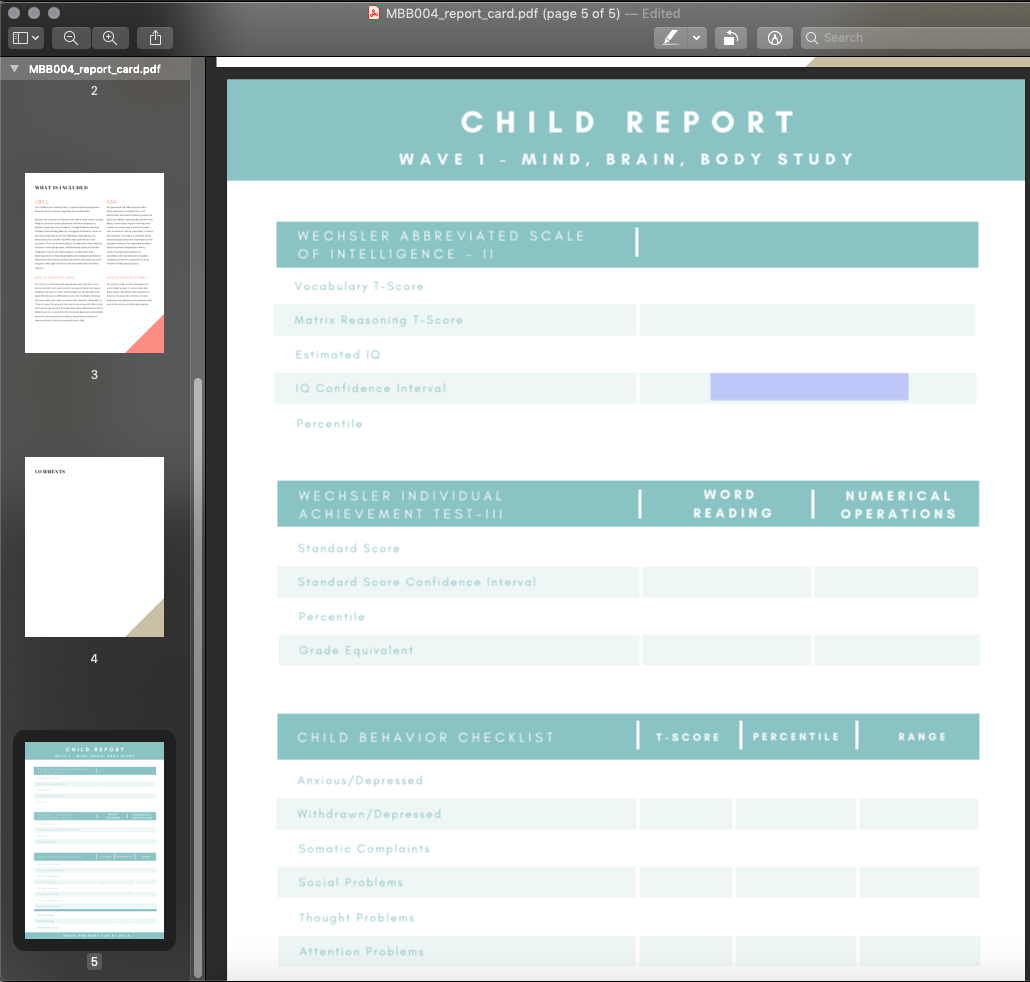
\includegraphics{images/final_checklist/report_cards/4.png}
\caption{}
\end{figure}

\begin{enumerate}
\def\labelenumi{\arabic{enumi}.}
\setcounter{enumi}{4}
\tightlist
\item
  After you have entered the data, it should look like this
\end{enumerate}

\begin{figure}
\centering
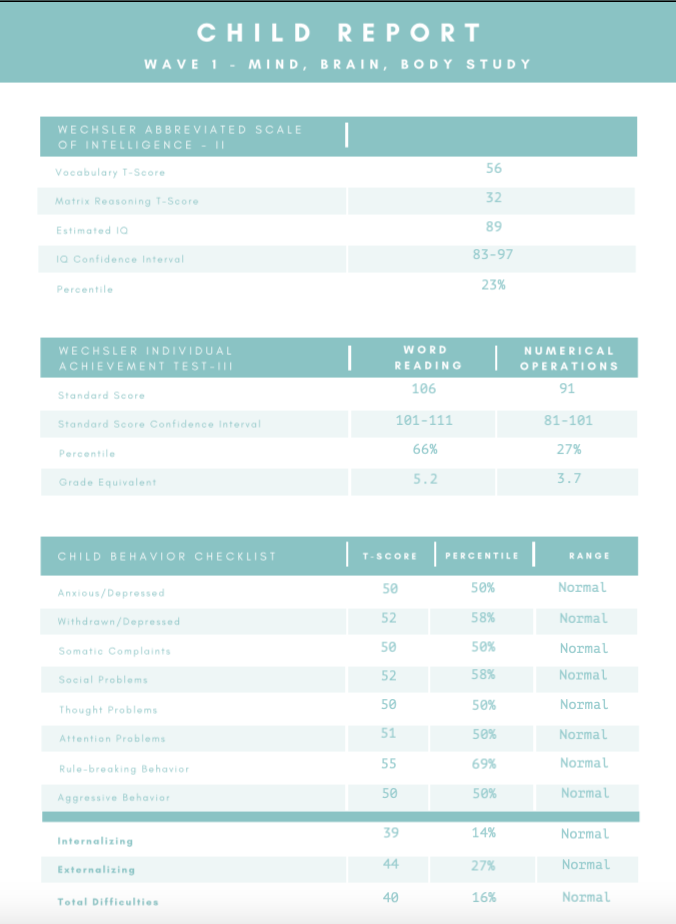
\includegraphics{images/final_checklist/report_cards/5.png}
\caption{}
\end{figure}

\begin{enumerate}
\def\labelenumi{\arabic{enumi}.}
\setcounter{enumi}{5}
\tightlist
\item
  If there are any comments, enter them on the comments page.
\end{enumerate}

\begin{itemize}
\item
  For example, if any NA's are present due to less than 70\% of data for that subset being available to calculate a score - note that here. Or, for example if the child was too young to receive a grade based score, you could note the aged based reading of the table here.
\item
  If there are no comments, delete this page.
\end{itemize}

\begin{figure}
\centering

\includegraphics{images/final_checklist/report_cards/6.png}
\caption{}
\end{figure}

\begin{enumerate}
\def\labelenumi{\arabic{enumi}.}
\setcounter{enumi}{6}
\tightlist
\item
  \textbf{Important} - Once you have completed the edits to the pdf, you must follow these steps to ``lock'' the data so that it is no longer editable before sending to the participant. To do so, click file/print/PDF/Save as PDF. Save the PDF to your desktop, then replace the original PDF with the desktop version.
\end{enumerate}

\begin{figure}
\centering
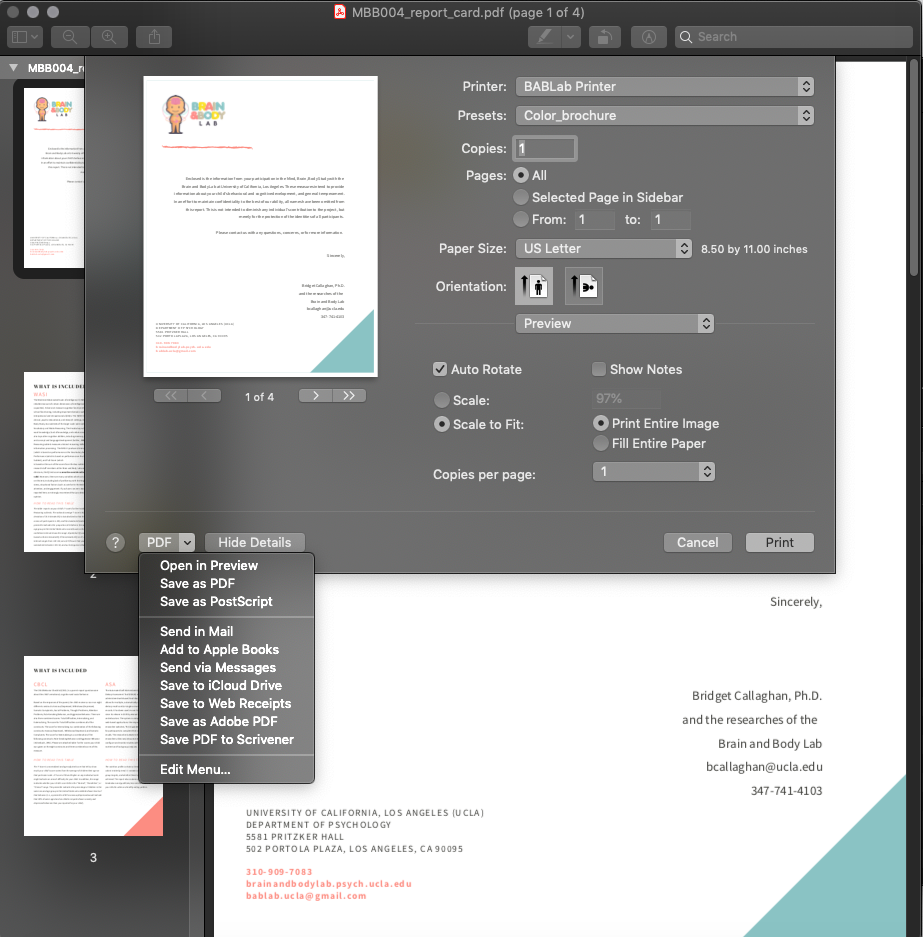
\includegraphics{images/final_checklist/report_cards/7.png}
\caption{}
\end{figure}

\begin{enumerate}
\def\labelenumi{\arabic{enumi}.}
\setcounter{enumi}{7}
\tightlist
\item
  The report card is now ready to be sent to the participant.
\end{enumerate}

\hypertarget{literature}{%
\chapter{Literature}\label{literature}}

Here is a review of existing methods.

Callaghan, B. L., Fields, A., Gee, D. G., Gabard-Durnam, L., Caldera, C., Humphreys, K. L., Goff, B., Flannery, J., Telzer, E. H., Shapiro, M., \& Tottenham, N. (2020). Mind and gut: Associations between mood and gastrointestinal distress in children exposed to adversity. Development and Psychopathology, 32(1), 309--328. \url{https://doi.org/10.1017/S0954579419000087}

(Callaghan et al., 2020)

\citep{xie2015}

\citep{callaghanMindGutAssociations2020a}

\bibliography{book.bib,packages.bib}


\end{document}
